\documentclass[11pt,a4paper]{article}

\usepackage[
    top    = 1in,
    right  = 1.5in,
    bottom = 1in,
    left   = 1.5in]{geometry}
\usepackage[utf8]{inputenc}
\usepackage[english]{babel}
\usepackage[T1]{fontenc}
\usepackage{lmodern}

\usepackage{amsmath,amssymb,amsfonts,float,subcaption,mathtools}

\title{Vision and Image Processing\\Assignment 4}
\author{Malte Stær Nissen    \\ \texttt{tgq958} \and
        Benjamin Braithwaite \\ \texttt{cpg608}}

\begin{document}
\maketitle

\section{Initial notes}
%
We have in this assignment implemented our own KLT tracker for tracking patches
throughout video sequences and will in this report first describe how the
tracker is implemented and then test the tracker on a couple of video sequences.
Finally we will comment on the results and shortly discuss ways of improving the
tracker.
%
\section{Kanade-Lucas-Tomasi (KLT) tracker}
%
As explained above we have implemented a KLT tracker. The tracker is built for
tracking fixed sized patches in video sequences. The main idea behind the
tracker algorithm is to estimate a displacement vector for each of the patches we
wish to track. We first assume the image change to be linear making us able to
model the image by a truncated Taylor series using only first order information.

Given a patch we now want to be able to compute the image displacement which
minimizes the squared intensity difference at the patch position in two
subsequent images. This is done by differentiating the residue expression which
leads us to compute a $2\times2$ matrix $G$ and the vector $\boldsymbol{e}$ being the residue
projected onto the gradient for each patch in the image.
\begin{align*}
    G &\approx \sum_{x \in W}
        \begin{bmatrix}
                g_x^2(x)      & g_x(x) g_y(x) \\
                g_x(x) g_y(x) & g_y^2(x)
        \end{bmatrix} w(x) \\
    e &\approx \sum_{x \in W}
    \begin{bmatrix}
        (I(x) - J(x)) g_x(x) w(x) \\
        (I(x) - J(x)) g_y(x) w(x)
    \end{bmatrix}
\end{align*}
Where $I$ is the current image and $J$ is the next image, and $g_x$ and
$g_y$ are the first order derivatives of $I$. We chose $w(x) = 1$ for
simplicity and we utilize the first order of the Gaussian distribution with
standard deviation $\sigma$ to first smooth and then derive our images in one
convolution (one for each direction).

Hereafter we compute the eigenvalues of $G$. Since $G$ is a $2 \times 2$ matrix,
we can compute the eigenvalues by solving the 2nd degree polynomial we
get from using the property of eigenvalues that:
\begin{align*}
    \text{det}\left( \lambda I - G\right) &= 0 \\
\end{align*}
Hereafter we filter the patches by only keeping those patches having their
lowest eigenvalue $min(\lambda_1,\lambda_2) > t_{init}$ where $t_{init}$ is the
initial threshold. This ensures that both eigenvalues are
sufficiently large and ensures that the patch contains a corner or texture.
Furthermore we only keep non-overlapping patches. This is done by sorting the patches by their
lowest eigenvalue in descending order and walking through the list from the top
throwing away a patch if it overlaps with one of the patches we already decided
to keep.

This detection of patches (implemented in \texttt{get\_features.mi}) could be
performed in all iterations but we haven chosen only do it in the first and then to
try to track the initial features for as long as possible.

When we have the filtered features we compute the estimate of the image
displacement of each patch by computing $G^{-1} \boldsymbol{e}$ where $G^{-1}$
is the pseudo-inverse of $G$ in order to avoid computing the inverse of a close
to singular matrix.
Having computed the displacement the first time, we now want to refine the exact
location of the patch in between pixels. We do this by interpolating the image
values using a bilinear interpolation of the coordinates of the new patch. We
do this for $i$ iterations in order to come up with the best estimate of patch
position. If we should've followed the original KLT algorithm we should've
performed this looping until convergence of the residue value or throw away the
patch if it didn't converge. We chose not to implement this part exactly as
intended due to time pressure before and during the exam period.

When performing the computation of the displacement we furthermore throw away
any patches that leaves the image including those who only partically overlap
with the image boundaries.

We now have the new estimates of the positions of our original patches and use
these estimates as the new patch in the next iteration. When running the
algorithm we use the initial threshold $t_{init}$ for thresholding the initial
patch candidates by their lowest eigenvalue. In the following iterations we use
a lower threshold $t_{keep}$ to filter away tracked patches which might have
diverged away from their correct position.
%
\section{Testing}
%
We test our tracker on the provided dudekface image sequence using the best
parameters we have found: $\sigma = 2$, 15x15 patch size, initial threshold
of $3 \cdot 10^{-4}$, keep threshold of $3 \cdot 10^{-6}$, and 5 convergence
iterations. Selected frames with the tracked feature patches and displacement
vectors are shown in Figure \ref{fig:tracker_dudekface}.
%
\begin{figure}[H]
    \centering
    \begin{subfigure}{0.45\textwidth}
        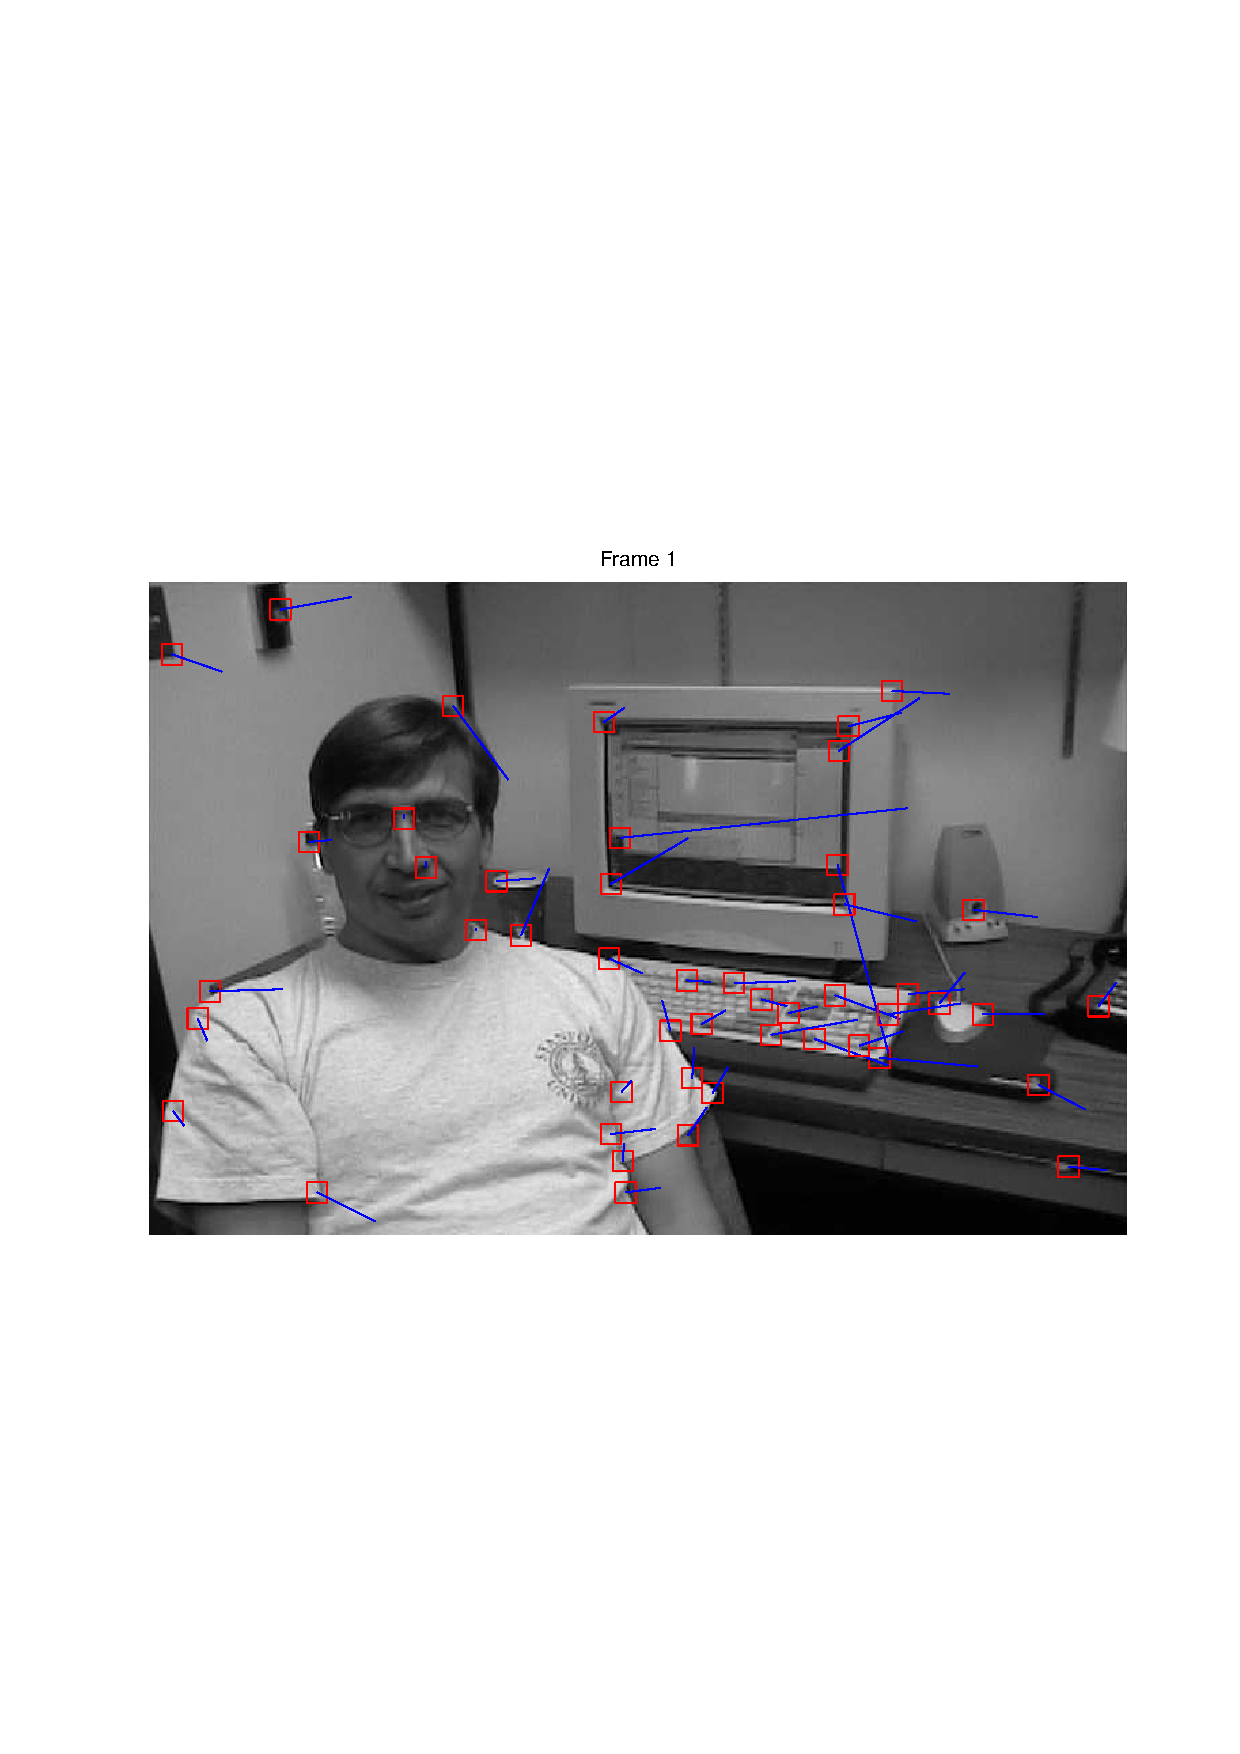
\includegraphics[scale=0.4,trim={120 250 0 250}]{img/tracker_dudekface_1.pdf}
    \end{subfigure}
    \begin{subfigure}{0.45\textwidth}
        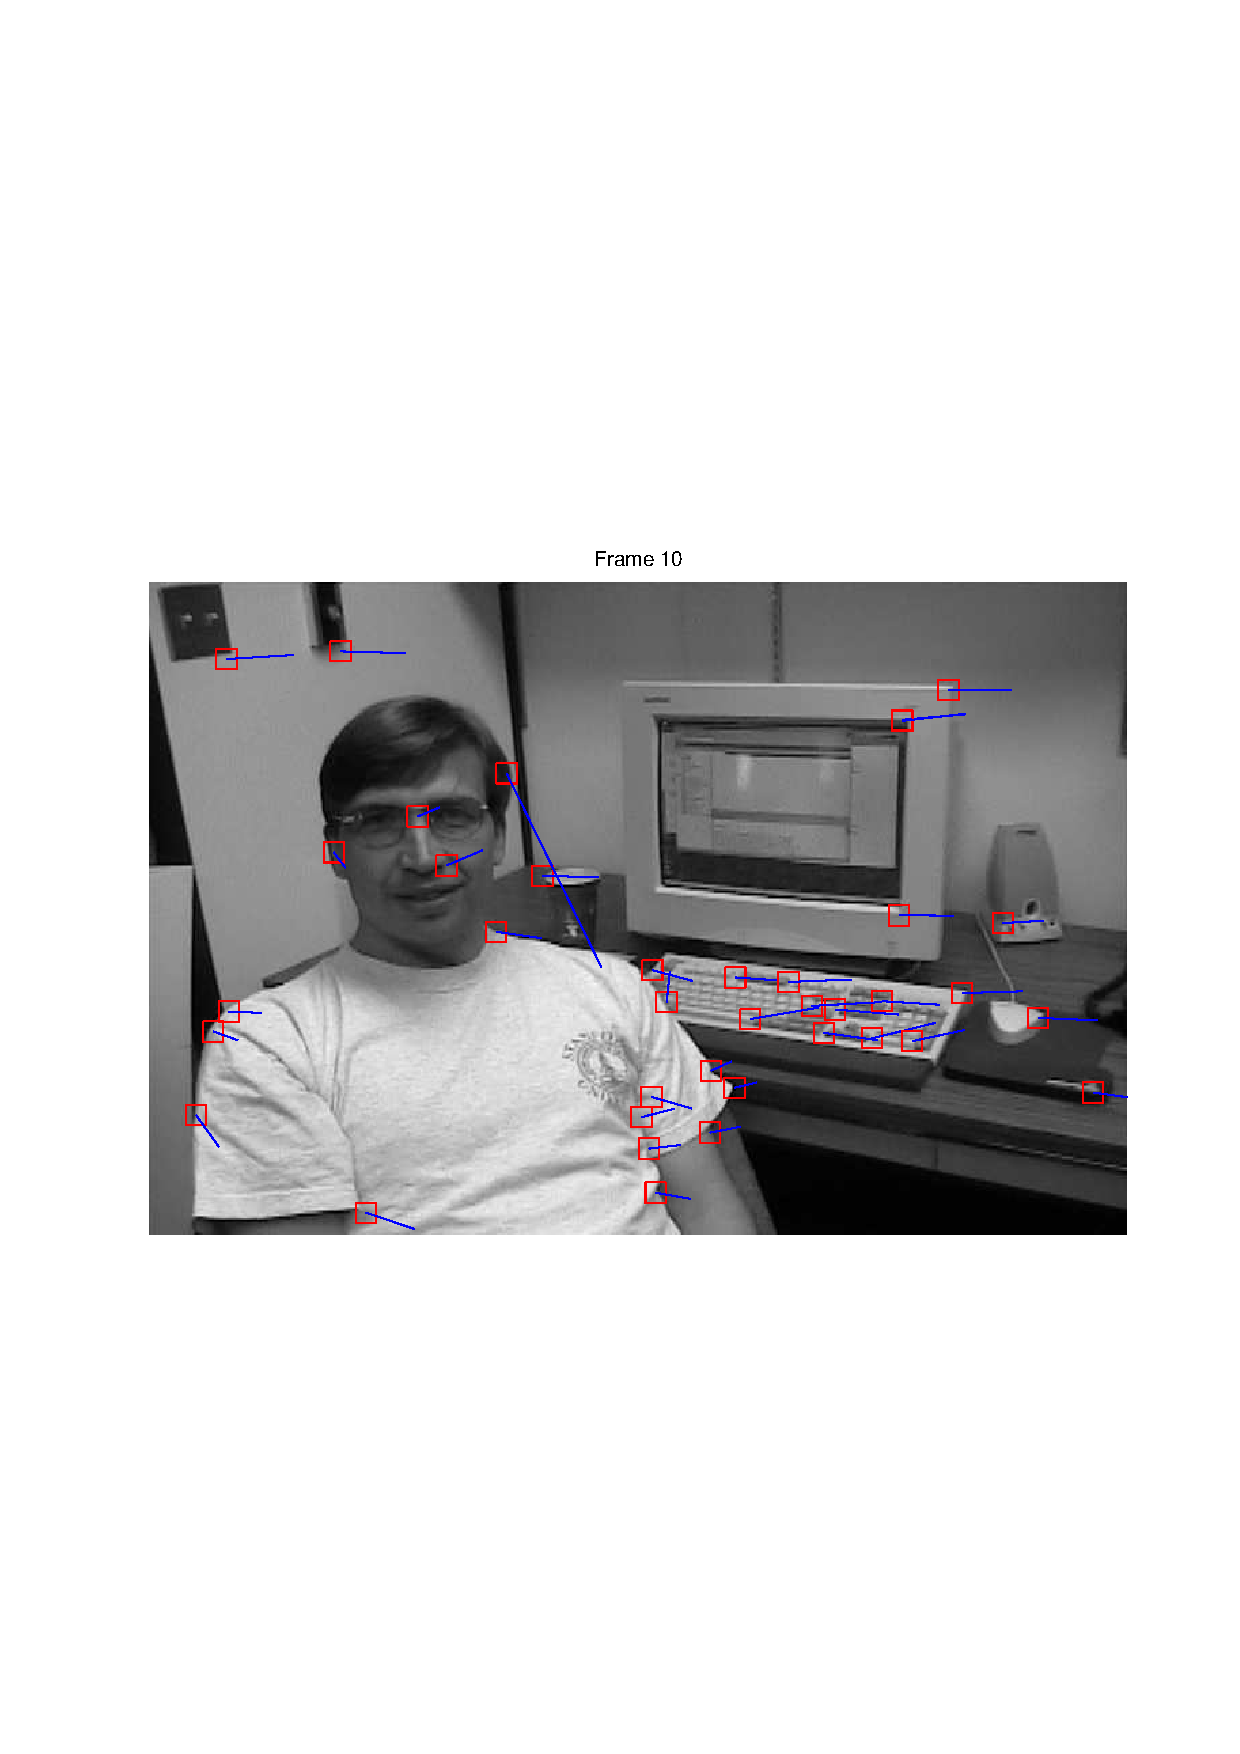
\includegraphics[scale=0.4,trim={70 250 0 250}]{img/tracker_dudekface_10.pdf}
    \end{subfigure}
    \begin{subfigure}{0.45\textwidth}
        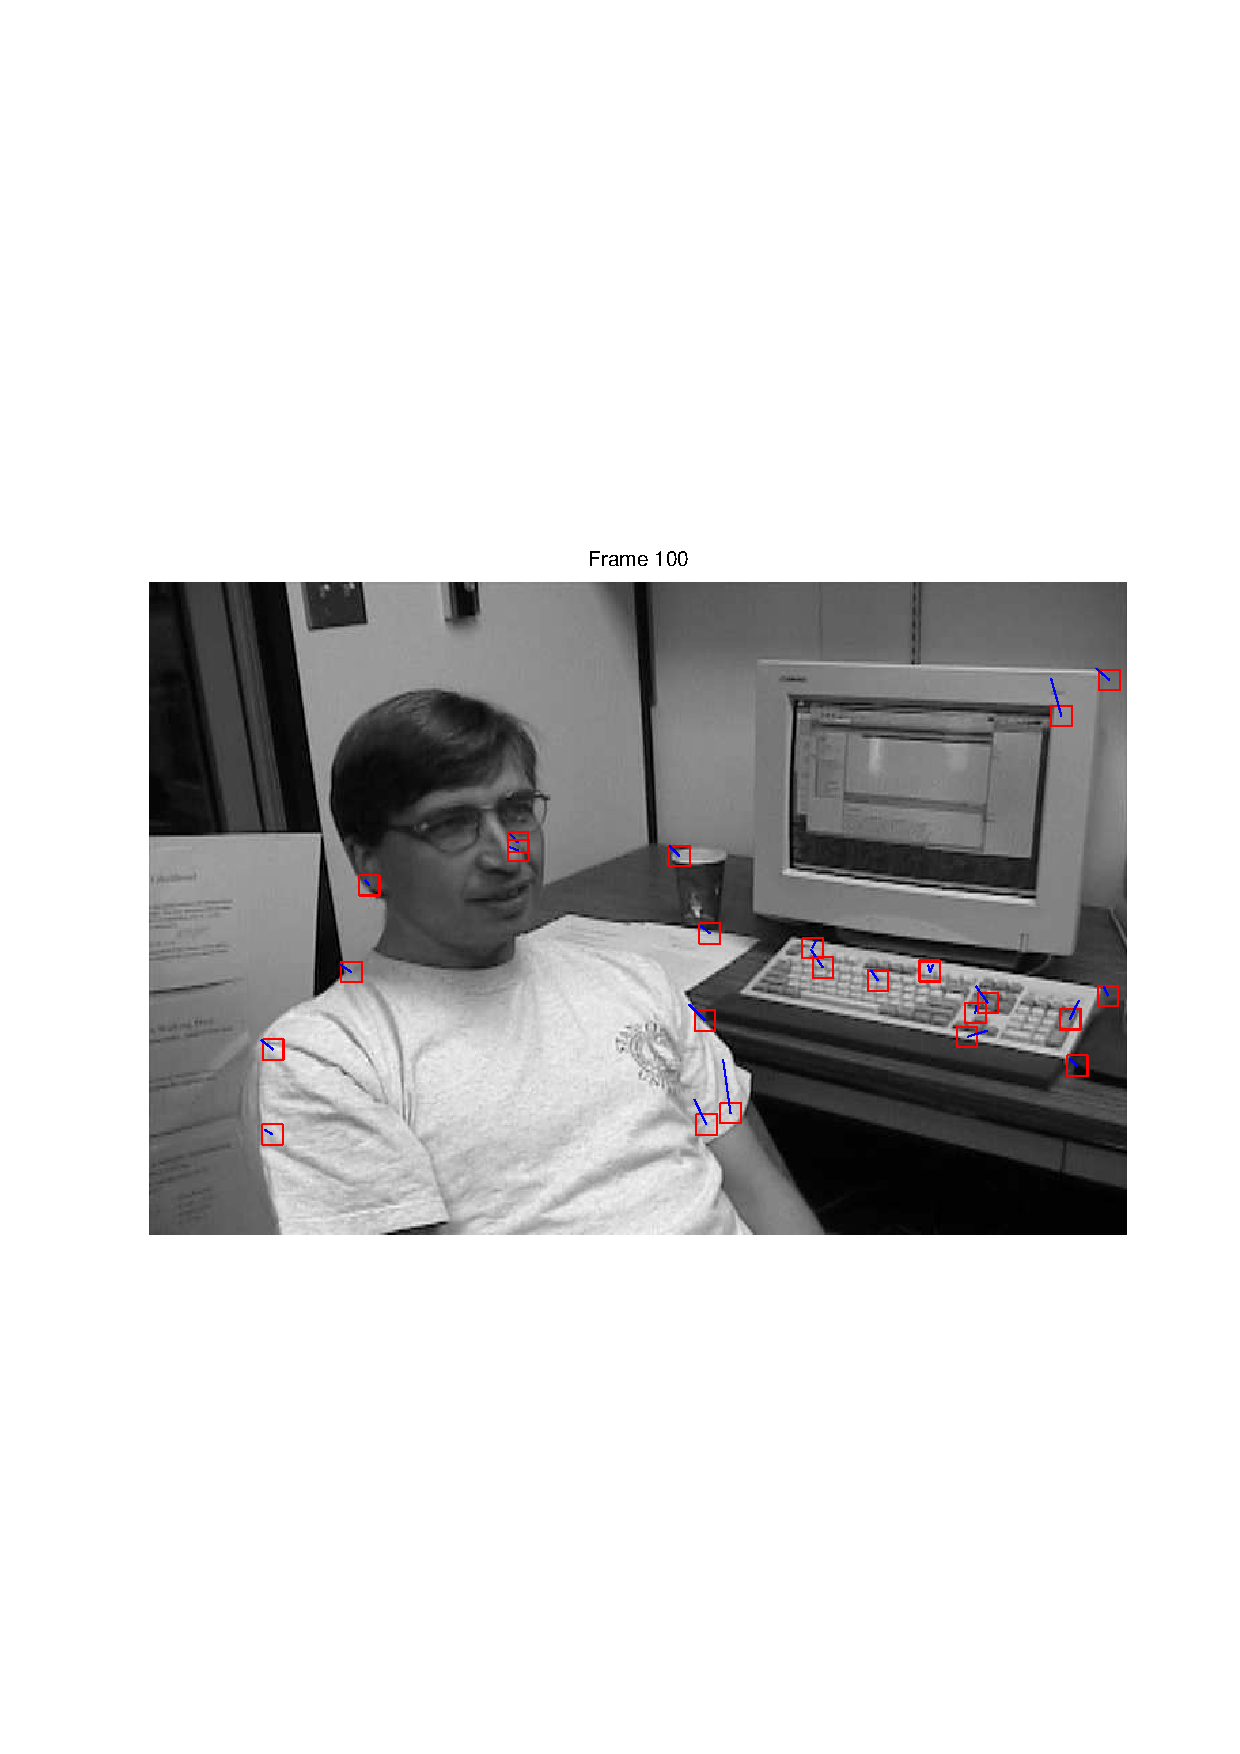
\includegraphics[scale=0.4,trim={120 250 90 250}]{img/tracker_dudekface_100.pdf}
    \end{subfigure}
    \begin{subfigure}{0.45\textwidth}
        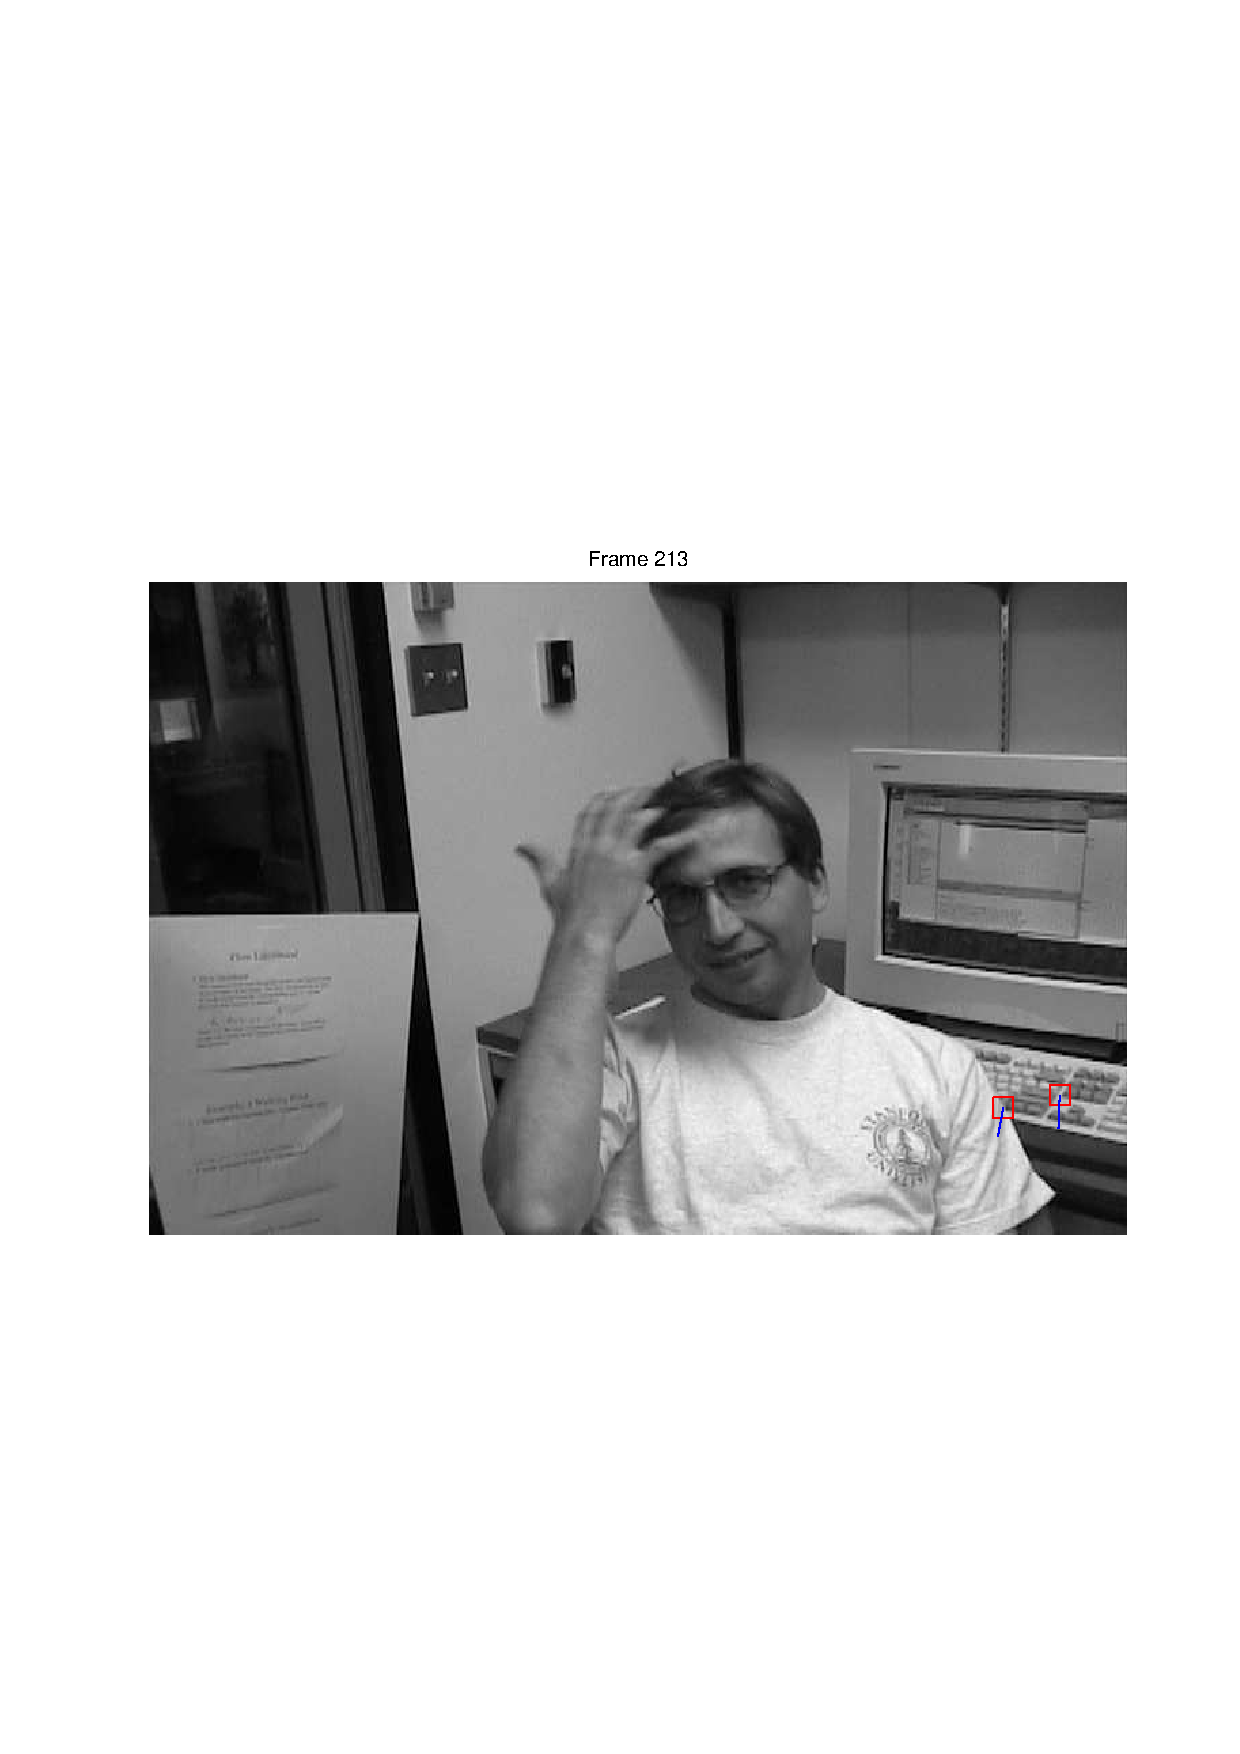
\includegraphics[scale=0.4,trim={70 250 90 250}]{img/tracker_dudekface_213.pdf}
    \end{subfigure}
    \caption{Frames 1, 10, 100 and 231 from our KLT tracker used on the
        dudekface image sequence. Feature patches are shown in red and (scaled)
        displacement vectors for these in blue.}
    \label{fig:tracker_dudekface}
\end{figure}

\end{document}

